% !TEX TS-program = pdflatex
% !TEX encoding = UTF-8 Unicode

% Compile with: pdflatex doski.tex

\documentclass[10pt]{article} % use larger type; default would be 10pt

\usepackage[utf8]{inputenc} % set input encoding (not needed with XeLaTeX)

\usepackage{siunitx}
\usepackage{hyperref}

%%% PAGE DIMENSIONS
\usepackage{geometry} % to change the page dimensions
\geometry{a4paper} % or letterpaper (US) or a5paper or....
\geometry{margin=2cm} % for example, change the margins to 2 inches all round
% \geometry{landscape} % set up the page for landscape
%   read geometry.pdf for detailed page layout information

\usepackage{graphicx} % support the \includegraphics command and options
\graphicspath{ {../diagrams/}, {../time_diagrams/} }

% \usepackage[parfill]{parskip} % Activate to begin paragraphs with an empty line rather than an indent

%%% PACKAGES
\usepackage{booktabs} % for much better looking tables
\usepackage{array} % for better arrays (eg matrices) in maths
\usepackage{paralist} % very flexible & customisable lists (eg. enumerate/itemize, etc.)
\usepackage{verbatim} % adds environment for commenting out blocks of text & for better verbatim
\usepackage{subfig} % make it possible to include more than one captioned figure/table in a single float
% These packages are all incorporated in the memoir class to one degree or another...

%%% HEADERS & FOOTERS
\usepackage{fancyhdr} % This should be set AFTER setting up the page geometry
\usepackage{t1enc}
\usepackage[hungarian]{babel}
\pagestyle{fancy} % options: empty , plain , fancy
\renewcommand{\headrulewidth}{0pt} % customise the layout...
\lhead{}\chead{}\rhead{}
\lfoot{}\cfoot{\thepage}\rfoot{}

%%% SECTION TITLE APPEARANCE
\usepackage{sectsty}
\allsectionsfont{\sffamily\mdseries\upshape} % (See the fntguide.pdf for font help)
% (This matches ConTeXt defaults)

%%% ToC (table of contents) APPEARANCE
\usepackage[nottoc,notlof,notlot]{tocbibind} % Put the bibliography in the ToC
\usepackage[titles,subfigure]{tocloft} % Alter the style of the Table of Contents
\renewcommand{\cftsecfont}{\rmfamily\mdseries\upshape}
\renewcommand{\cftsecpagefont}{\rmfamily\mdseries\upshape} % No bold!

%%% END Article customizations

\title{Programozható LED-fűzéren alapuló reklámpanel - LED fűzér vezérlése, adatok kiírása}
\author{Patka Zsolt-András | Számítástechnika BSc}
\date{2019.11.11}

\begin{document}
\maketitle

\section{Beveztő}

A projekt célja egy LED-fűzér vezérlése és ennek segítségével egy reklámszöveg megjelenítése. Ehhez egy FPGA lap és egy Worldsemi WS2813 ledfűzér lesz felhasználva.

\section{Követelmények}

\subsection{Funkcionális követelmények}
\begin{itemize}
\item Lehetséges legyen egy reklámszöveget kiírni a ledfűzérek által létrehozott mátrix-ra.
\item Egy sorban minimum 100 LED található
\item Az egyes ledfűzérek szinkronba működjenek
\item A kiírás párhuzamosan történik az adott ledfűzéreken
\item Másodpercenként 60 frissítés (60 Hz)
\item Mozgó szöveg
\end{itemize}

\subsection{Nem funkcionális követelmények}
\begin{itemize}
\item Benti használatra van tervezve
\item Ha az FPGA-lapnak lesz készítve külön tokozat, akkor IP31-es standardnak kell megfeleljen
\item Ha az FPGA-lapnak nem lesz készítve külön tokozat, akkor nem felel meg IP standardnak (IP00)
\end{itemize}

\subsection{Fejlesztési követelmények}
\begin{itemize}
\item Implementáció VHDL nyelvben
\item Szimulációs állomány a rendszer tesztelésére
\item Adatok kiírása lehetséges a LED fűzérre
\item Modularitás
\begin{itemize}
	\item Külön modul egy 24 bit-es blokk küldésére
	\item Külön modul a 24 bit-es blokkokat küldő modulok használatára (paraméterezhető, bővíthető)
\end{itemize}
\item Opcionális: 
\begin{itemize}
	\item Pár betű kódolása (3-4)
	\item Betük tárolása BRAM memóriában
\end{itemize}
\end{itemize}

\section{Rendszer-specifikáció}

\begin{itemize}
\item WS2813 egyszálú adatátvitel protokolljának helyes használata
\item Worldsemi WS2813 100 LED-es ledfűzér van felhasználva
\item Digilent Basys3 FPGA vezérli a ledfűzért 
\end{itemize}

\section{Tervezés}


\subsection{WS2813 egyszálú adatátvitel protokoll leírása}

\indent A LED-eket vezérlő áramkörök egymás után vannak bekötve úgy, hogy az egyik áramkörnek az adatkimenete a következő áramkörnek az adatbemenetét képzi. Egyszálú az adatátvitel, fontos a protokoll betartása, ahhoz, hogy adatokat tudjunk megjeleníteni a LED-fűzéren.

Amikor egy áramkör megkap egy 24 bit-es kódot, akkor ezt addig tárolja amíg más kódot nem kap, vagy a tápforrást el nem veszti.

\subsubsection{A 24 bit-es kód}

A 24 bit-es kód a következőképpen kell kinézzen:

8 bit GREEN | 8 bit RED | 8 bit BLUE

Az adatátvitel a következő sorrendben kell történjen: 
\begin{enumerate}
	\item GREEN
	\item RED
	\item BLUE
\end{enumerate}

\subsubsection{Bit-ek küldési sorrendje}

\textbf{Az egyes byte-ok küldését úgy kell elvégezni, hogy az MSB-vel kell kezdeni és haladni az LSB fele.}

\noindent 24 bit-es kód részletesebb felbontása: 
\begin{itemize}
\item \textit{G7 G6 G5 G4 G3 G2 G1 G0 | R7 R6 R5 R4 R3 R2 R1 R0 | B7 B6 B5 B4 B3 B2 B1 B0}
\end{itemize}

\noindent A küldés a következő sorrendben kell elvégződjön: 
\begin{itemize}
\item \textbf{G7 G6 G5 G4 G3 G2 G1 G0 | R7 R6 R5 R4 R3 R2 R1 R0 | B7 B6 B5 B4 B3 B2 B1 B0}
\end{itemize}

\subsubsection{Időzítések}

Minden 24 bit-es adatátvitel után kell legalább \SI{50}{\micro\second}-ot várakozni, alacsony feszűltségen. Ez jelzi azt, hogy egy 24 bit-es blokk továbbítása megtörtént.

\noindent Az egyes bit-ek átvitele a következőképp történik:

\begin{itemize}
\item Logikai 1-es
	\begin{itemize}
	\item \SI{0.8}{\micro\second}-ot magas feszűltségen
	\item \SI{0.45}{\micro\second}-ot alacson feszűltségen
	\end{itemize}
\item Logikai 0-ás
	\begin{itemize}
	\item \SI{0.4}{\micro\second}-ot magas feszűltségen
	\item \SI{0.85}{\micro\second}-ot alacson feszűltségen
	\end{itemize}
\item 24 bit-es adatblokk küldése után: 
	\begin{itemize}
		\item $ > \SI{50}{\micro\second}$-ot alacsony feszűltségen
	\end{itemize}
\end{itemize}

\noindent A bit-ek továbbításánál egy +/- \SI{150}{\nano\second}-os eltérés megengedett.

A várakozási értékeket nem az adatlapból, hanem az \href{https://learn.adafruit.com/adafruit-neopixel-uberguide}{alábbi} útmutatóból vettem. Az útmutató szerint az adatlapban levő értékek rosszul vannak kiszámolva.

Egyelőre megpróbálok az útmutatóban megadott értékekkel dolgozni. Ha ez nem megfelelő működéshez vezet, akkor veszem az adatlapban levő értékeket.


\subsection{Véges állapotú adatútas automata tervezése}

A feladatot egy véges állapotú adatútas automatával fogom megoldani. Ennek megfelelően mutatom be a tervezést.

\subsubsection{Elvégezendő RT műveletek azonosítása}

Az időzítések implementálásához egy számláló lesz használva. A 100 MHz-es órajel ami fel lesz használva időben $\SI{0.01}{\micro\second}$-nak felel meg. 
Így a szükséges ciklusok száma (amennyit várakoztatni kell bizonyos feszűltségszinten, ahhoz, hogy a WS2813 protokollja be legyen tartva) egész.
Ebből már látható, hogy definiálható két művelet: $i \Leftarrow ciklus\_szam$, $i \Leftarrow i - 1$ (ahol i a számláló).

\indent Az egyszerűség kedvéért, egy belső regiszternek, amely a színadatokat tartalmazza (\textbf{data}), mindig a 24. bitje kerül kiküldésre.
Tehát minden bit kiküldése után ennek a regiszternek az értékeit el kell csúsztatni (shift-elni) egyet balra: $data \Leftarrow data << 1$

\indent Egy 24-bites blokk kiküldése után kell küldeni egy "RES" jelet, vagyis több ideig alacsony feszűltségen kell tartani a kimenetet. 
Ehhez számolni kell a már elküldött bitek számát $bit\_count \Leftarrow bit\_count + 1$, ahol bit\_count az eddig elküldött bitek számát tartalmazza.

\subsubsection{Adatfüggőségek identifikálása}

Mivel nagyon egyszerű RT műveletekkel meg lehet oldani az adott feladatot, nem merűlnek fel adatfüggőségek.

\subsubsection{Célregiszterek azonosítása}

Szükséges regiszterek:
\begin{itemize}
	\item $R_i$: ciklusszámláló regiszter a késleltetésekhez.
	\item $R_{bit}$\_count: Biteket számláló regiszter, a 24 bit-es blokk elküldésének érzékeléséhez.
	\item $R_{data}$: Elkündendő adatot tartalmazó regiszter
\end{itemize}

\subsubsection{Különböző fázisokban elvégzendő műveletek}

\begin{table}[h!]
	\begin{center}
		\caption{Különböző fázisokban elvégzendő műveletek}
		\begin{tabular}{l|c|c|c|c|c}
		\textbf{Állapot} & $R_i$ 	 & $R_{bit\_count}$     & $R_{data}$      & d\_out 	 & done \\
		\hline         
		READY            & $R_i$ 	 & $R_{bit\_count}$     & $R_{data}$      & 'U' 	 & '0' \\
		\hline         
		INIT          	 & $R_i$ 	 & $R_{bit\_count}$     & $R_{data}$      & 'U' 	 & $done$ \\
		\hline         
		SEND\_IF01       & $R_i$ 	 & $R_{bit\_count}$     & $R_{data}$      & 'U' 	 & $done$ \\
		\hline         
		SEND1H\_INIT  	 & $T1H$ 	 & $R_{bit\_count}$     & $R_{data}$      & '1' 	 & $done$ \\
		\hline         
		SEND1H           & $R_i - 1$ & $R_{bit\_count}$     & $R_{data}$      & $d\_out$ & $done$ \\
		\hline         
		SEND1L\_INIT     & $T1L$     & $R_{bit\_count}$     & $R_{data}$      & '0'      & $done$ \\
		\hline         
		SEND1L           & $R_i - 1$ & $R_{bit\_count}$     & $R_{data}$      & $d\_out$ & $done$ \\
		\hline         
		SEND0H\_INIT     & $T0H$     & $R_{bit\_count}$     & $R_{data}$      & '1'      & $done$ \\
		\hline         
		SEND0H           & $R_i - 1$ & $R_{bit\_count}$     & $R_{data}$      & $d\_out$ & $done$ \\
		\hline         
		SEND0L\_INIT     & $T0L$     & $R_{bit\_count}$     & $R_{data}$      & '0'      & $done$ \\
		\hline         
		SEND0L           & $R_i - 1$ & $R_{bit\_count}$     & $R_{data}$      & $d\_out$ & $done$ \\
		\hline
		SHIFT\_CHECK     & $R_i$     & $R_{bit\_count} + 1$ & $R_{data} << 1$ & $d\_out$ & $done$ \\
		\hline
		SENDRES\_INIT    & $TRES$    & $R_{bit\_count}$     & $R_{data}$      & '0'      & $done$ \\
		\hline
		SENDRES          & $R_i - 1$ & $R_{bit\_count}$     & $R_{data}$      & $d\_out$ & $done$ \\
		\hline
		SEND\_DONE       & $R_i$ 	 & $R_{bit\_count}$     & $R_{data}$      & 'U' 	 & '1' \\
		\hline
		DONE\_TODO       & $R_i$ 	 & $R_{bit\_count}$     & $R_{data}$      & 'U' 	 & $done$ \\
		\end{tabular}
	\end{center}
\end{table}

\subsection{Állapotok}

\textbf{2019.10.14}

Állapotok:
\begin{itemize}
\item READY
	\begin{itemize}
	\item Alap állapot 
	\item "reset" jel esetén ide kerül vissza az automata
	\end{itemize}
\item INIT
	\begin{itemize}
	\item minden LED-et kikapcsol (0x000000-t ír)
	\item "clear" jel esetén ide kerül az automata
	\end{itemize}
\item RENDER
	\begin{itemize}
	\item egyenként küldi a szín információt a LED-ekre
	\item annyiszor végződik el itt a művelet, ahány LED-ünk van
	\item "stop" jel esetén megáll a kiírás
	\end{itemize}
\item DISPLAY
	\item megtörtént a kiírás
\end{itemize}

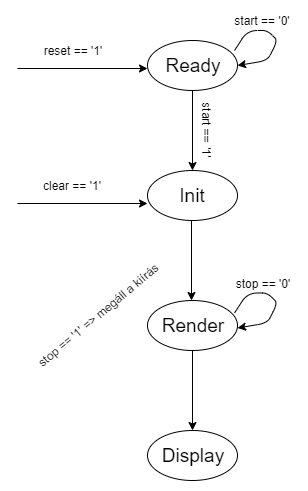
\includegraphics[scale=0.5]{allapotdiagram.png}

\textbf{2019.10.28}

Állapotdiagram átírva úgy, hogy a küldési logikát is tartalmazza:

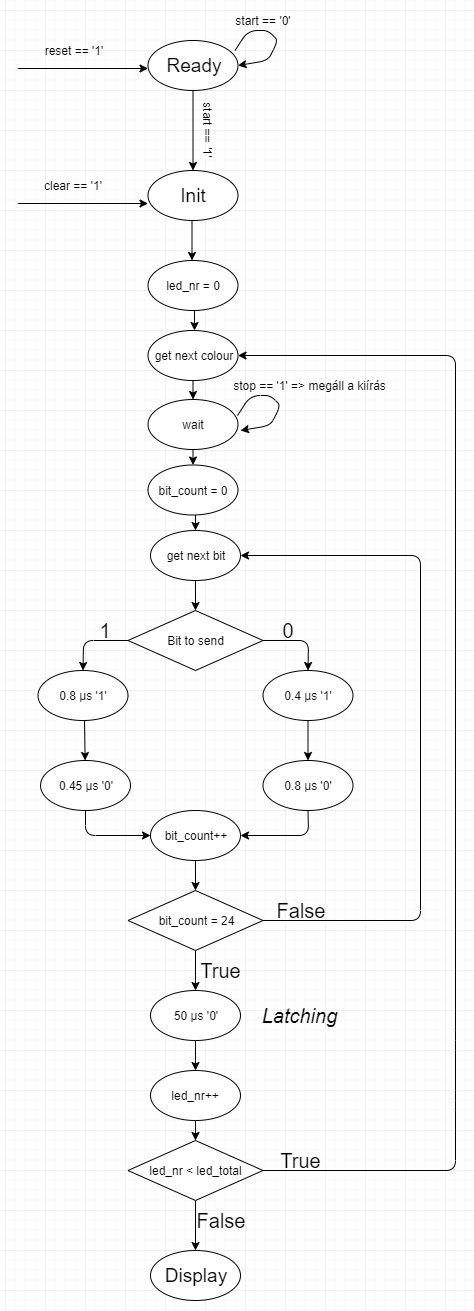
\includegraphics[scale=0.4]{allapotdiagram_2.png}

Állapotdiagram egy 100 LED-et vezérlő modulra

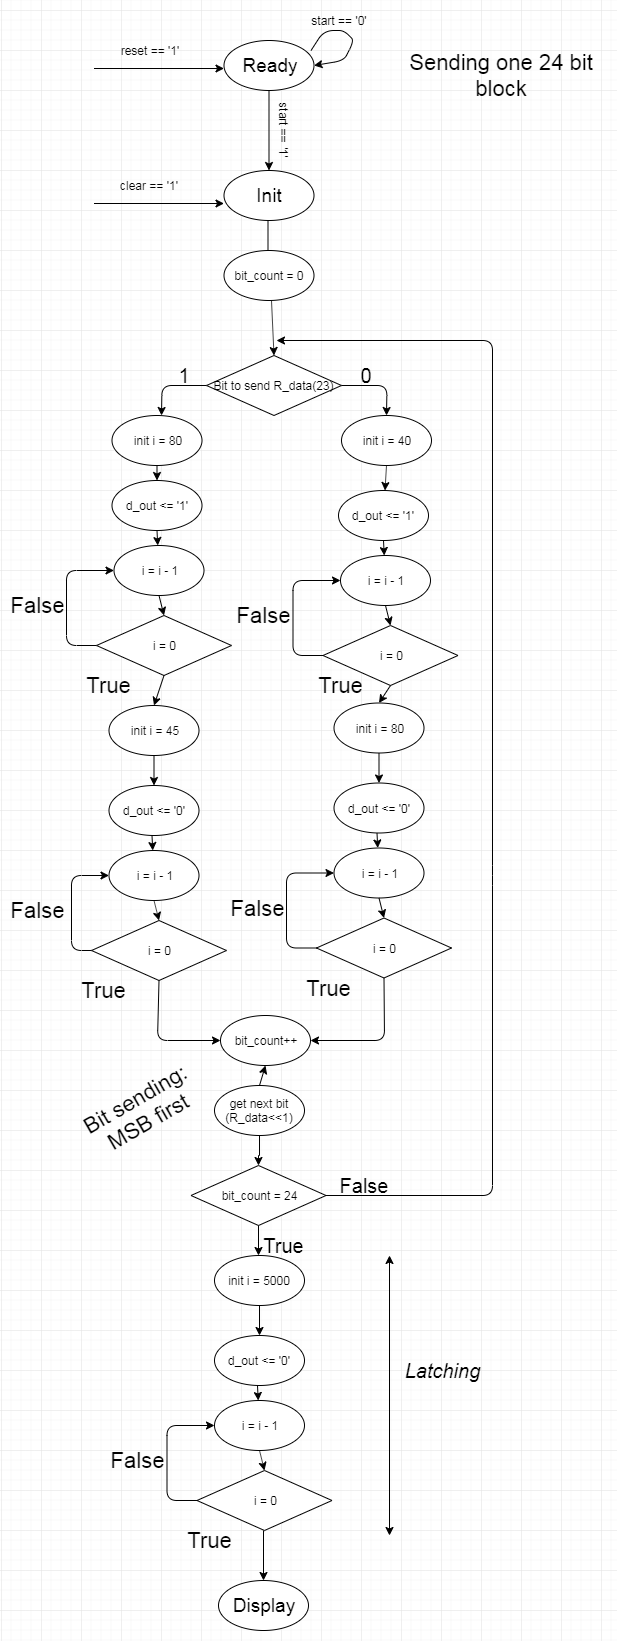
\includegraphics[scale=0.4]{allapotdiagram_3.png}

\textbf{2019.11.11}

Végleges állapotdiagram, az implementációban is használt.

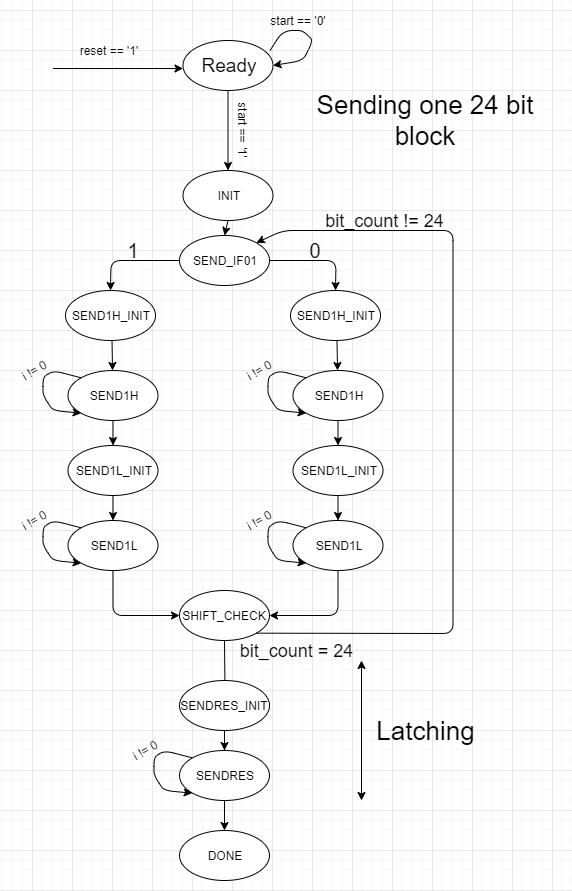
\includegraphics[scale=0.5]{allapotdiagram_final.png}

\begin{itemize}
\item READY
	\begin{itemize}
	\item Alap állapot 
	\item "reset" jel esetén ide kerül vissza az automata
	\end{itemize}
\item INIT
	\begin{itemize}
	\item inicializálja a bit-count-ot nullára
	\end{itemize}
\item SENDIF\_01
	\begin{itemize}
	\item Megvizsgálja data[23]-as bit-et. Ha 1, akkor a következő állapot a \textbf{SEND1H\_INIT}, ha 0 akkor SEND0H\_INIT
	\end{itemize}
\item SEND1H\_INIT
	\begin{itemize}
	\item Inicializálja az \textbf{i} változót a T1H értékre
	\item A d\_out output-ot 1-re állítja
	\end{itemize}
\item SEND1H
	\begin{itemize}
	\item Dekrementálja az \textbf{i} változót
	\item Amikor az \textbf{i} változó nulla lesz, akkor tovább megy a \textbf{SEND1L\_INIT} állapotra
	\end{itemize}
\item SEND1L\_INIT
	\begin{itemize}
	\item Inicializálja az \textbf{i} változót a T1L értékre
	\item A d\_out output-ot 0-ra állítja
	\end{itemize}
\item SEND1L
	\begin{itemize}
	\item Dekrementálja az \textbf{i} változót
	\item Amikor az \textbf{i} változó nulla lesz, akkor tovább megy a \textbf{SHIFT\_CHECK} állapotra
	\end{itemize}
\item SEND0H\_INIT
	\begin{itemize}
	\item Inicializálja az \textbf{i} változót a T0H értékre
	\item A d\_out output-ot 1-re állítja
	\end{itemize}
\item SEND0H
	\begin{itemize}
	\item Dekrementálja az \textbf{i} változót
	\item Amikor az \textbf{i} változó nulla lesz, akkor tovább megy a \textbf{SEND0L\_INIT} állapotra
	\end{itemize}
\item SEND0L\_INIT
	\begin{itemize}
	\item Inicializálja az \textbf{i} változót a T0L értékre
	\item A d\_out output-ot 0-ra állítja
	\end{itemize}
\item SEND0L
	\begin{itemize}
	\item Dekrementálja az \textbf{i} változót
	\item Amikor az \textbf{i} változó nulla lesz, akkor tovább megy a \textbf{SHIFT\_CHECK} állapotra
	\end{itemize}
\item SHIFT\_CHECK
	\begin{itemize}
	\item Megnézi, hogy a \textbf{bit\_count} változó 24-e, ha igen, akkor tovább megy a \textbf{SENDRES\_INIT} állapotra
	\item Ha a \textbf{bit\_count} változó nem egyenlő 24-el, akkor shift-eli a \textbf{data} std logic vectort balra eggyel; vissza megy a \textbf{SEND\_IF01} állapotra
	\end{itemize}
\item SENDRES\_INIT
	\begin{itemize}
	\item Inicializálja az \textbf{i} változót a TRES értékre
	\item A d\_out output-ot 0-ra állítja
	\end{itemize}
\item SENDRES
	\begin{itemize}
	\item Dekrementálja az \textbf{i} változót
	\item Amikor az \textbf{i} változó nulla lesz, akkor tovább megy a \textbf{SEND\_DONE} állapotra
	\end{itemize}
\item SEND\_DONE
	\begin{itemize}
	\item Befejeződött a 24 bit-es blokk kiírása
	\item Beállítja a \textbf{done} kimenetet 1-esre
	\end{itemize}
\end{itemize}

\subsection{Alegységek}

\textbf{2019.10.14}
\begin{itemize}
\item Következő állapot regiszter \textbf{\textit{Next State Register}}
\item Állapot regiszter \textbf{\textit{State Register}}
\item Szín regiszter \textbf{\textit{Colour Register}}
\item Küldési logika regiszter \textbf{\textit{Transmission Logic Register}}
\end{itemize}

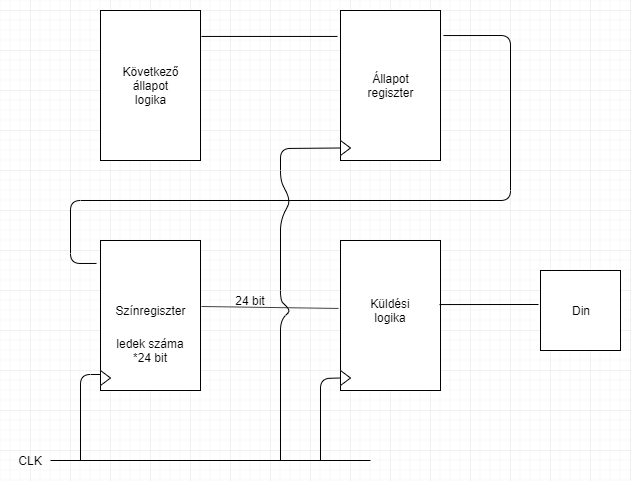
\includegraphics[scale=0.5]{tombvazlat.png}

\subsubsection{Küldési logika regiszter}

\noindent A küldési logika modul részletesebb lebontása: 

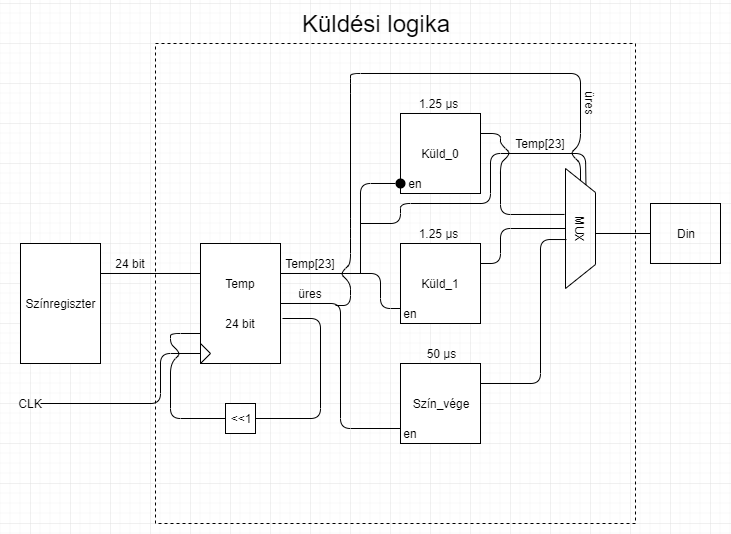
\includegraphics[scale=0.6]{kuldesi_logika.png}

\textbf{2019.10.28}

\indent Minden \textbf{led\_controll} modulhoz tartozik egy BRAM blokk és minden ilyen modul egy ledfűzért vezérel meg. Öt ilyen blokk megvezérel öt ledfűzért, ezáltal létrehozva a ledmátrixot.
Az órajel, start, reset, stop és data-rd jelek közösek minden modulnak.

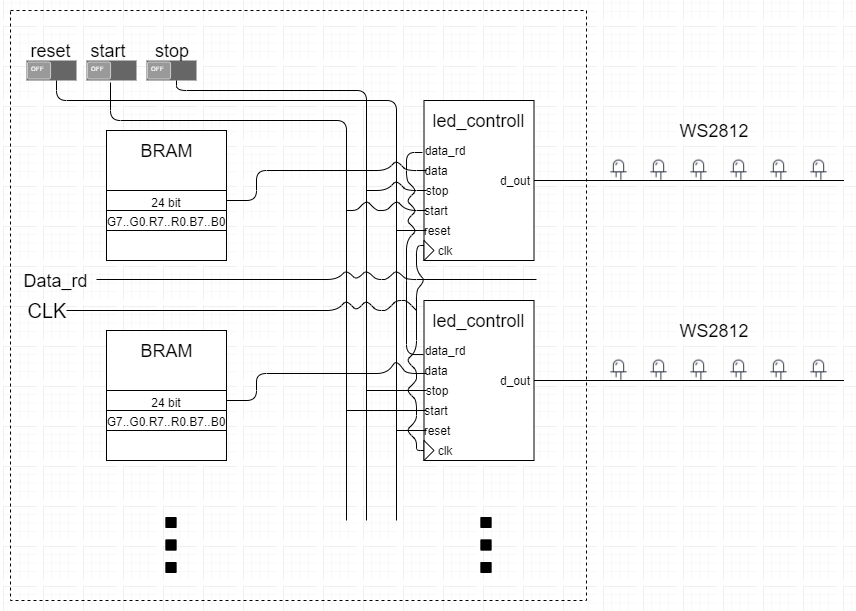
\includegraphics[scale=0.5]{tombvazlat2.png}




\subsection{Idődiagram}

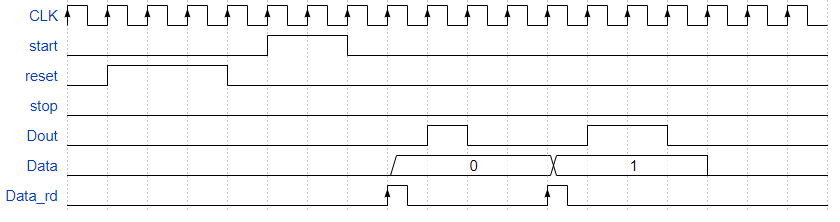
\includegraphics[scale=0.6]{general.PNG}

\begin{itemize}
\item CLK: 100 MHz-es órajel
\item start: jel a folyamat elindításához
\item reset: jel a folyamat resetálásához
\item stop: jel a kiírás megállításához. Csak két 24 bit-es blokk kiírása közben tudja megállítani a kiírást
\item Dout: Egyszálú adatsín a LED-ekre.
\item Data: Kiírandó adat, Data\_rd felmenő órajelére olvassa be az adatot.
\item Data\_rd: Aktiváló bit az adat beolvasására
\end{itemize}

\textbf{2019.11.11}

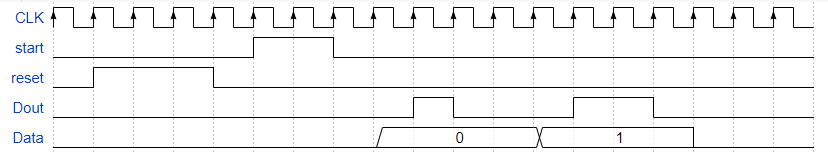
\includegraphics[scale=0.6]{general2.PNG}

\begin{itemize}
\item CLK: 100 MHz-es órajel
\item start: jel a folyamat elindításához
\item reset: jel a folyamat resetálásához
\item Dout: Egyszálú adatsín a LED-ekre.
\item Data: Kiírandó adat
\end{itemize}

\end{document}
